
\subsection*{Schedule of the Project}

Validating a simulation framework for all the possible applications listed above might be unfeasible for a single project. A tentative schedule, together with the tasks, is presented in Figure \ref{fig:sched}. It is composed of six main activities:

\begin{enumerate}
    \item adapter completion:
    \begin{itemize}
        \item verification of coupling step: the current version of the adapter \cite{caccia2021coupling}  proved to be much faster and more robust to added mass instability \cite{van2009added} than the original one, but it requires a redundant MBDyn computation. It can be optimized, possibly impacting the MBDyn code.
        \item completion of integration with preCICE: some features need to be completed 
    \end{itemize}

    \item validation: 
    \begin{itemize}
        \item some experimental benchmarks are available \cite{heathcote2008effect}: the mitigation of mesh deformation and distortion \cite{de2007mesh} needs to be analyzed
        \item suitable aeroelastic benchmarks must be found 
    \end{itemize}
    
    \item implementation of a controlled rigid model and comparison with experimental data 
    
    \item implementation of an aeroservoelastic model and comparison with experimental data
    
    \item implementation of new features in MBDyn: a sort of ``inverse kinematics" with respect to the logic described in \cite{quaranta2005conservative}, with the goal to perform hybrid multi-body full finite element co-simulation. Some ideas can possibly be mutuated by \texttt{rbe2} or \texttt{rbe3} elements.

    \item implementation of new features in the adapter: e.g.\ inserting a new displacement layer  between the multi-body model displacements and the interface displacements, to perform shape morphing (keeping the structural properties constant)
    
\end{enumerate}


\begin{landscape}

\begin{figure}
\centering
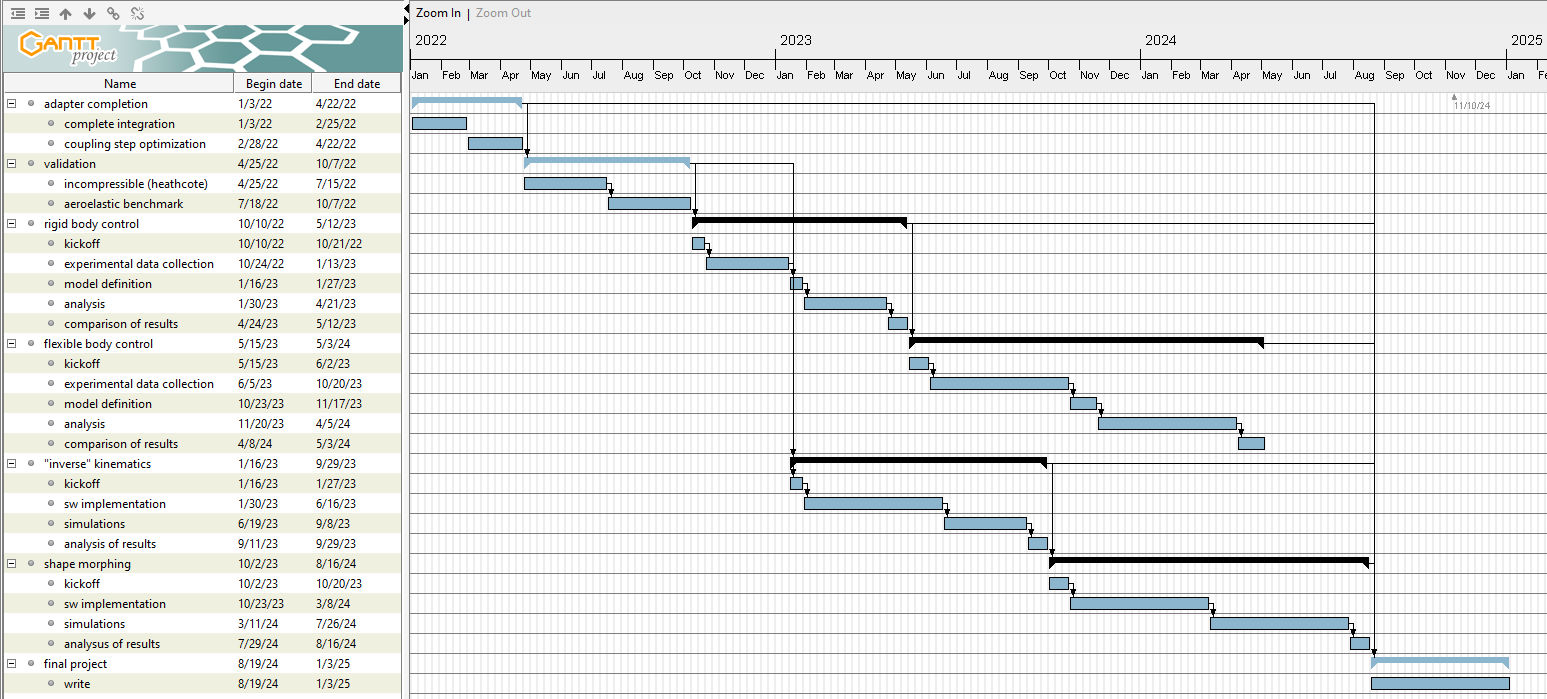
\includegraphics[width=1.6\textwidth]{images/Gantt_PhD.PNG}
\caption{Project schedule.}
\label{fig:sched}
\end{figure}

\end{landscape}

